\subsection{Inteligencia Artificial}

El método racional fusiona la ingeniería y las matemáticas basándose en las "leyes del pensamiento", las cuales tienen su origen en la antigua Grecia y han sido influenciadas por filósofos como Aristóteles. Durante el siglo XIX, se diseñaron programas capaces de resolver problemas de lógica. Por consiguiente, el propósito de la Inteligencia Artificial en la vida real es crear sistemas inteligentes que posean estas habilidades. Aun en situaciones de incertidumbre, un "Agente Racional" toma acciones con el fin de obtener el mejor resultado posible. La inteligencia artificial se apoya en diversas disciplinas, tales como la ingeniería computacional, la teoría de control, la cibernética, la lingüística, la filosofía, la economía, la psicología, la neurociencia y las matemáticas, de acuerdo con \cite{bk_russell2004intart}.

Dos investigadores en neurociencia crearon el primer modelo de IA basado en neuronas artificiales en 1943, dando inicio al análisis de la Inteligencia Artificial. McCulloch y Pitts idearon el prototipo que permitía que las neuronas fueran <<activadas>> o <<desactivadas>>, lo que demostró que una red de neuronas era capaz de realizar cualquier tarea computacional. Posteriormente, Donald Hebb propuso la <<Regla de Aprendizaje Hebbiano>>. John McCarthy, Allen Newell y Herbert Simon desarrollaron un programa que podía tener el pensamiento no numérico en el taller de Dartmouth, aunque no se publicó. El término <<Inteligencia Artificial>> fue acuñado por McCarthy, \parencite{bk_russell2004intart}.

La IA comenzó a entrar en la industria en los años 80, especialmente en grandes empresas de países desarrollados, a través de la investigación en sistemas expertos y el desarrollo de computadoras más poderosas.

\subsection{Aprendizaje Automático}
El Machine Learning es un área de la Inteligencia Artificial enfocada en técnicas que permiten a las computadoras aprender a través de algoritmos, convirtiendo muestras de datos en programas sin requerir programación explícita. Según \cite{bk_russell2009intart}, el aprendizaje automático es una división de la inteligencia artificial. Estos algoritmos emplean tecnologías como el procesamiento del lenguaje natural, el aprendizaje profundo y las redes neuronales. Tanto el aprendizaje supervisado como el no supervisado se fundamentan en lecciones extraídas de los datos. La creación de algoritmos capaces de recibir datos de entrada y utilizar análisis estadístico para prever una salida, la cual se ajusta conforme se obtienen nuevos datos, constituye el fundamento del aprendizaje automático. \parencite{bk_alpaydin2014ml}

Se puede clasificar en cuatro tipos principales de la siguiente manera según el objetivo que se desea alcanzar mediante el uso de ML:
\begin{itemize}
	\item \textbf{Aprendizaje Supervisado}: El Aprendizaje Supervisado se ganó su nombre porque los científicos de datos actúan como una guía para enseñarle al algoritmo las conclusiones a las que debe llegar. Es similar a la forma en que un estudiante aprende aritmética básica de un maestro. Este tipo de aprendizaje requiere datos etiquetados con las respuestas correctas que se esperan del resultado del algoritmo. Para problemas de clasificación y regresión, el aprendizaje supervisado demostró ser preciso y rápido según \parencite{bk_zambrano2018supnosup}.
	
	Los dos tipos de Aprendizaje Supervisado son:

	\begin{itemize}
		\item \textbf{Clasificación}: es la predicción del valor categórico de salida que permite dividir los datos en clases específicas. La clasificación se puede usar para varios propósitos, como determinar el clima, determinar si un correo electrónico es spam o no o identificar tipos de animales después de recibir una educación adecuada, un conjunto de datos con etiquetas de imágenes que incluyen la especie y algunas identificaciones características, según \parencite{bk_zambrano2018supnosup}.
		\item \textbf{Regresión}: es un tipo de problema en el que la predicción de un valor de respuesta continua es necesaria, como los precios de las acciones y la vivienda, según \parencite{bk_zambrano2018supnosup}.
	\end{itemize}

	Por lo tanto, funciona modelando las relaciones y dependencias entre las características de entrada y la salida de predicción objetivo, lo que permite predecir los valores de salida para nuevos datos utilizando las relaciones que aprendió de conjuntos de datos anteriores, según \parencite{bk_alpaydin2014ml}.

	\item \textbf{Aprendizaje No Supervisado}: Por otro lado, el Aprendizaje No Supervisado se asemeja más a lo que algunos expertos llaman Inteligencia Artificial real: la idea de que una máquina puede aprender a identificar patrones y procesos complejos sin la supervisión de humanos. Cuando los expertos no saben qué buscar en los datos y los datos en sí no incluyen objetivos, este método es particularmente útil. La agrupación de k-means, el análisis de componentes principales e independientes y las reglas de asociación según \parencite{bk_zambrano2018supnosup} son algunos de los muchos casos de uso del Aprendizaje Automático No Supervisado.
	
	\begin{itemize}
		\item \textbf{Agrupación K-means}: es un tipo de problema en el que cosas similares están agrupadas, como se muestra en la Figura \ref{2:fig12}. Comparte el mismo concepto con la clasificación, pero no se proporcionan etiquetas, por lo que el sistema entenderá los datos y los agrupará. Un uso de esto sería agrupar los artículos y las noticias según su género y contenido, según \parencite{tec_sancho2018supnosup}
	\end{itemize}
	
		\begin{figure}[H]
		\begin{center}
			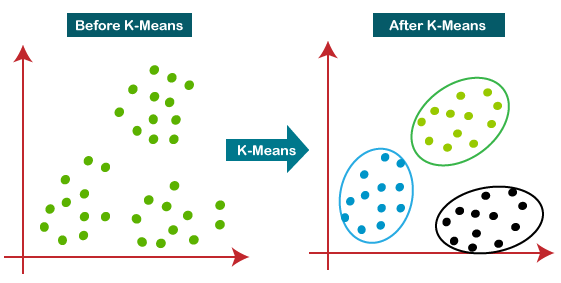
\includegraphics[width=0.75\textwidth]{2/figures/kmeans.png}
			\caption[El algoritmo de K medias]{El algoritmo de K medias.\\
			Fuente: \cite{tec_sancho2018supnosup}. \citetitle{tec_sancho2018supnosup}.}
			\label{2:fig12}
		\end{center}
	\end{figure}
		
	Debido a su complejidad y dificultad de implementación, este tipo de Aprendizaje Automático no se utiliza tan frecuentemente como el Aprendizaje Supervisado, a pesar de que abre las puertas a la resolución de problemas que los humanos normalmente no abordarían, según \parencite{tec_sancho2018supnosup}

	\item \textbf{Aprendizaje Semisupervisado}: Hasta el momento, todos los datos enviados han sido etiquetados con el resultado deseado o no han sido etiquetados en absoluto. El Aprendizaje Automático Semisupervisado utiliza ambos. El costo de etiquetar es bastante alto en muchas situaciones prácticas y, en el caso de grandes conjuntos de datos, se vuelve aburrido y requiere mucho tiempo. Además, proporcionar demasiados datos etiquetados puede hacer que el modelo tenga sesgos humanos. A pesar de que los datos sin etiquetar son desconocidos para la red, ofrecen información útil sobre los parámetros del grupo objetivo. que conduce a la conclusión de que se puede mejorar la precisión del modelo al incluir datos sin etiquetar y, al mismo tiempo, ahorrar tiempo y dinero en su construcción. Por ejemplo, la clasificación de páginas web, el reconocimiento de voz o la secuenciación genética pueden usar Aprendizaje Automático Semisupervisado. En esos casos, los científicos de datos pueden acceder a grandes cantidades de datos sin etiquetarlos, y la tarea de etiquetarlos todos llevaría mucho tiempo, según \parencite{bk_zambrano2018supnosup}.

	Se puede comparar estos tres tipos de Aprendizaje Automático para el mismo uso, como clasificación, utilizando los datos recopilados hasta ahora:

	\begin{itemize}
		\item \textbf{Clasificación supervisada}: el algoritmo clasificará los tipos de páginas web según las etiquetas proporcionadas desde el principio, según \parencite{bk_zambrano2018supnosup}.
		\item \textbf{Agrupación no supervisada}: el algoritmo buscará patrones y características que ayudan a agrupar páginas web en grupos, según \parencite{bk_zambrano2018supnosup}.
		\item \textbf{Clasificación semi no supervisada}: identificará varios grupos de páginas web utilizando los datos etiquetados, luego utilizará los datos no etiquetados para establecer los límites de esos grupos de páginas web y buscar otros tipos que posiblemente no aparezcan en los datos etiquetados, según \parencite{bk_zambrano2018supnosup}.
	\end{itemize}
	
\end{itemize}

\subsection{Aprendizaje Profundo}

Desde que llegó la Inteligencia Artificial hace un tiempo, tiene una amplia gama de aplicaciones y se divide en muchas ramas, como se menciona en \parencite{gl_sas_deeplearning}. El Aprendizaje Profundo es un subconjunto del Aprendizaje Automático, que es en sí mismo un subcampo de la IA. La Figura \ref{2:fig13} es una representación visual de la relación entre AI, ML y DL.

\begin{figure}[H]
	\begin{center}
		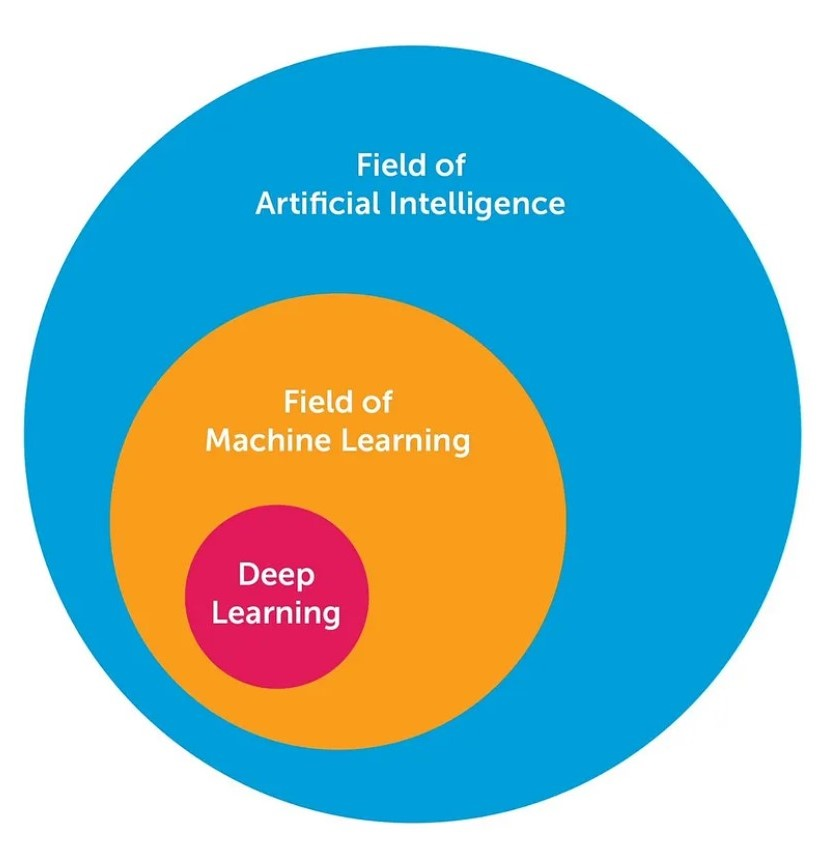
\includegraphics[width=0.50\textwidth]{2/figures/deeplearning_machinelearning.jpg}
		\caption[Relación entre IA, ML y DL]{Relación entre IA, ML y DL.\\
		Fuente: \cite{tec_cook2018deeplearning}. \textit{Most Popular 20 Free Online Courses to Learn Deep Learning}.}
		\label{2:fig13}
	\end{center}
\end{figure}

El Aprendizaje Profundo no solo permite representar datos de la manera correcta, sino que también permite que la computadora aprenda programas informáticos de varios pasos al incluir el concepto de profundidad en sus modelos. Como se muestra en la Figura \ref{2:fig14}, cada capa de representación puede interpretarse como el estado de la memoria de la computadora. Las computadoras interpretan las imágenes como una colección de valores de píxeles que representan escenas de nuestra realidad. Según \parencite{tec_cook2018deeplearning}, identificar un objeto o mapear su identidad a partir de esos valores es una tarea difícil para las máquinas y puede resultar casi imposible cuando se intenta aprender este mapeo directamente.

\begin{figure}[H]
	\begin{center}
		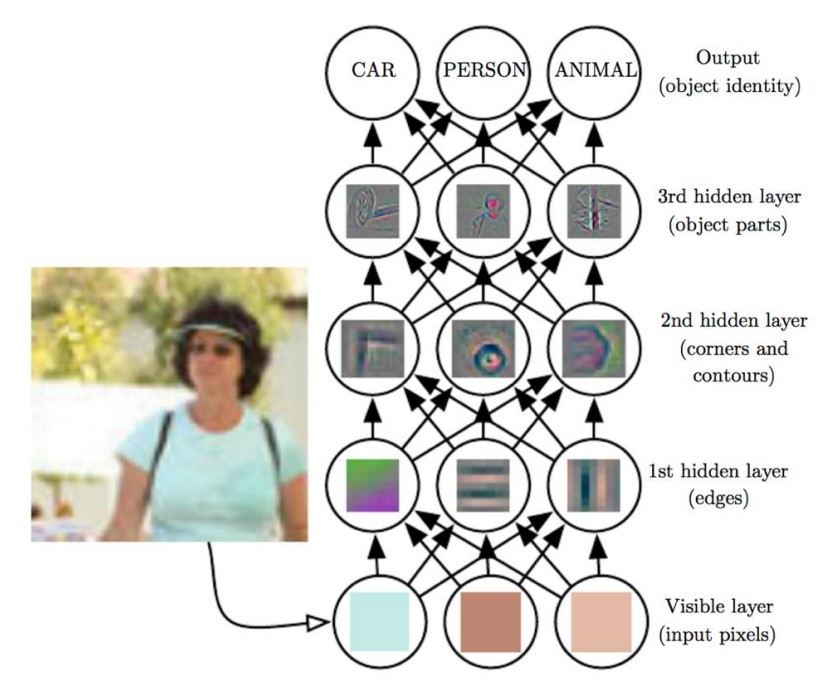
\includegraphics[width=0.70\textwidth]{2/figures/deeplearning_machinelearning2.jpg}
		\caption[Modelo de aprendizaje profundo]{Modelo de aprendizaje profundo.\\
		Fuente: \cite{tec_cook2018deeplearning}. \textit{Most Popular 20 Free Online Courses to Learn Deep Learning}.}
		\label{2:fig14}
	\end{center}
\end{figure}


\subsection{Segmentación de Imágenes}
%%%%%%%%
\subsubsection{Definición y objetivos de la segmentación de imágenes}
La segmentación de imágenes es un proceso fundamental en el campo del procesamiento de imágenes y la visión por computadora, cuyo propósito es dividir una imagen en partes significativas y coherentes, facilitando su análisis e interpretación. Este proceso busca simplificar la representación de una imagen, destacando las regiones de interés o los objetos específicos que contiene, separándolos del fondo y otras áreas irrelevantes. \parencite{gonzalez2018}

Los objetivos principales de la segmentación incluyen identificar, clasificar y delimitar regiones u objetos dentro de una imagen. En aplicaciones prácticas, estos objetivos son cruciales, ya que permiten resolver problemas como la detección de bordes, la identificación de patrones, la localización de estructuras específicas y el análisis morfológico. En el ámbito médico, por ejemplo, la segmentación de imágenes se utiliza para identificar tejidos, órganos o anomalías, como tumores o lesiones. De manera similar, en la industria cosmética, este proceso puede emplearse para detectar características faciales como arrugas y manchas, ayudando en la evaluación estética y la personalización de tratamientos. \parencite{gonzalez2018}

Existen múltiples técnicas para la segmentación, que van desde enfoques tradicionales como la segmentación basada en umbrales, el análisis de regiones y la detección de bordes, hasta métodos avanzados como las redes neuronales convolucionales (CNN). Estas últimas han revolucionado el campo al permitir segmentaciones más precisas y automáticas, especialmente en imágenes complejas donde las características pueden ser sutiles o con variaciones significativas en color, textura y forma. Por ello, la segmentación es un paso esencial en cualquier flujo de trabajo que involucre el análisis de imágenes, proporcionando una base sólida para tareas más avanzadas de procesamiento y análisis. \parencite{gonzalez2018}
%%%%%%
\subsubsection{Importancia de la segmentación en aplicaciones médicas y cosméticas}
En el ámbito médico y cosmético, la segmentación precisa de imágenes juega un papel crucial al permitir que los profesionales de la salud y la belleza realicen evaluaciones más detalladas y personalizadas de las condiciones dermatológicas. Este proceso facilita la identificación y el análisis de características específicas de la piel, lo que es fundamental para detectar anomalías y personalizar los tratamientos de acuerdo con las necesidades individuales de los pacientes o clientes. La segmentación es particularmente importante en el diagnóstico de enfermedades de la piel, donde la capacidad de identificar y analizar estructuras o patrones morfológicos específicos puede mejorar significativamente la precisión del diagnóstico.

Por ejemplo, en dermatología, la segmentación adecuada de imágenes faciales permite identificar con mayor precisión imperfecciones cutáneas como manchas y arrugas. Estos elementos son indicadores comunes de diversas afecciones dermatológicas, como el envejecimiento prematuro, las manchas solares o los trastornos hormonales. De igual manera, en la industria cosmética, la segmentación de características faciales es esencial para el diseño de tratamientos personalizados, ayudando a los profesionales a ofrecer soluciones más efectivas que aborden las preocupaciones estéticas específicas de cada cliente.

El uso de técnicas avanzadas de segmentación, como las redes neuronales convolucionales (CNN), ha revolucionado el campo, permitiendo una segmentación más precisa y automatizada, incluso en casos complejos donde las características de la piel pueden ser sutiles o variar en color, textura o forma. La segmentación no solo mejora la detección de condiciones dermatológicas, sino que también optimiza la personalización de tratamientos cosméticos, ya que permite que los productos sean aplicados de manera más eficiente, dirigiéndose específicamente a las áreas que requieren intervención. Esto puede resultar en un mejor rendimiento de los productos cosméticos, mayor satisfacción del cliente y, en última instancia, en una mejora de la salud de la piel.

En resumen, la segmentación de imágenes en el ámbito médico y cosmético no solo mejora la capacidad de diagnóstico, sino que también facilita la personalización de tratamientos, mejorando la efectividad y la satisfacción de los pacientes o clientes. \parencite{mohammadi2019}
%%%%%%%%%
\subsubsection{Técnicas de segmentación clásicas y sus limitaciones en imágenes dermatológicas}
Las técnicas clásicas de segmentación, como el umbralizado y la detección de bordes, han sido fundamentales en los primeros enfoques de procesamiento de imágenes. Estas técnicas buscan dividir la imagen en regiones homogéneas basadas en características como el color, la intensidad de los píxeles o los bordes de los objetos. Sin embargo, en el contexto dermatológico, estas técnicas presentan limitaciones significativas debido a la complejidad y variabilidad inherente de las imágenes de la piel.

Una de las técnicas clásicas más utilizadas es el \textit{umbralizado}, que divide una imagen en dos o más regiones basadas en el valor de intensidad de los píxeles. Esta técnica es eficiente cuando los objetos a segmentar se destacan claramente del fondo. Sin embargo, en imágenes dermatológicas, la piel tiene una amplia gama de tonalidades y texturas que varían entre diferentes personas, lo que puede dificultar la aplicación de umbrales estáticos que funcionen de manera efectiva en todos los casos. Además, las variaciones en la iluminación y la presencia de sombras en la piel pueden afectar negativamente el rendimiento del umbralizado, llevando a una segmentación incorrecta de las áreas de interés, como las arrugas o manchas.

La \textit{detección de bordes}, otra técnica clásica, se utiliza para identificar discontinuidades en la imagen, donde los bordes de los objetos se encuentran con un contraste significativo con el fondo. Técnicas como el operador de Sobel o el Canny se han utilizado para detectar bordes en imágenes de la piel. Sin embargo, los bordes de las características cutáneas no siempre están claramente definidos. La piel puede tener bordes suaves o difusos, especialmente cuando se trata de características como manchas o líneas finas. Esto hace que la detección de bordes sea menos efectiva para segmentar detalles sutiles en la piel, lo que limita su capacidad para proporcionar una segmentación precisa.

Estas técnicas clásicas también presentan dificultades cuando se enfrentan a características dermatológicas con variaciones complejas en la textura y el color de la piel. Por ejemplo, las manchas pueden tener bordes poco definidos, y las arrugas pueden ser de diferente grosor y profundidad. Además, las características morfológicas de la piel, como las arrugas finas, pueden tener formas irregulares que no se ajustan bien a las suposiciones que estas técnicas clásicas requieren. Las técnicas basadas en umbrales o en la detección de bordes también son sensibles al ruido y pueden ser ineficaces al trabajar con imágenes con poca calidad o cuando las características de la piel tienen un contraste bajo con el fondo.

Debido a estas limitaciones, las técnicas clásicas de segmentación no siempre son adecuadas para aplicaciones dermatológicas de alta precisión. Aunque siguen siendo útiles en ciertos contextos, su capacidad para segmentar con precisión detalles finos en la piel es insuficiente cuando se requiere una segmentación detallada y robusta. Es por esto que, en los últimos años, las técnicas más avanzadas, como las redes neuronales convolucionales (CNN), han comenzado a ganar popularidad en el campo de la dermatología y la cosmética, ofreciendo una solución más precisa y automática para la segmentación de características morfológicas complejas en la piel. \parencite{yoo2020}


\subsection{Redes Neuronales Convolucionales (CNN)}

Hoy en día, el procesamiento de imágenes, que incluye problemas de clasificación y visión por computadora, es una de sus aplicaciones más relevantes. El proyecto de Yann LeCun, ImageNet, utiliza el reconocimiento de objetos en imágenes.
	
Estas redes también se utilizan para clasificar textos. Ronan Collobert y Jason Weston modificaron la arquitectura y los parámetros internos de las Redes Neuronales Convolucionales para usarlas en aplicaciones del PLN. La Figura \ref{2:fig15} muestra la estructura de una CNN para problemas de procesamiento de información natural. \parencite{bk_kamath2019deeplearning_nlp_sr}
	
\begin{figure}[H]
	\begin{center}
		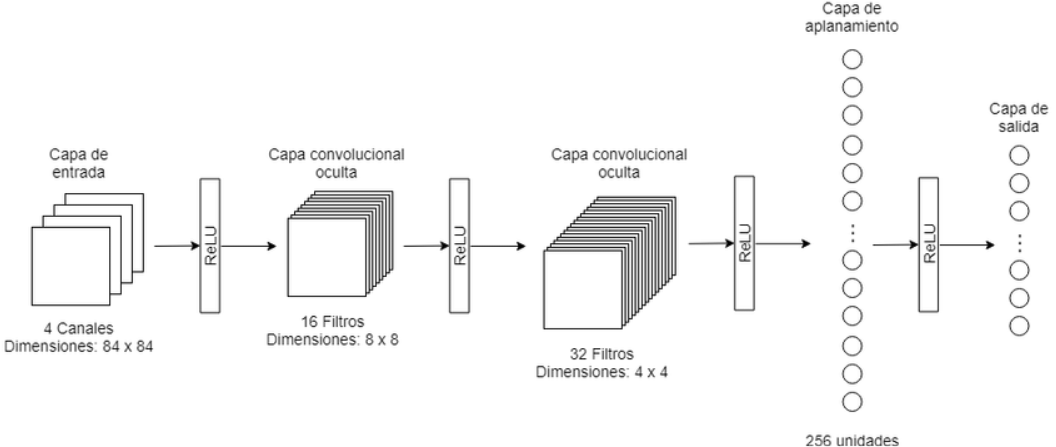
\includegraphics[width=0.95\textwidth]{2/figures/cnn_nlp.png}
		\caption[Arquitectura de un modelo CNN]{Arquitectura de un modelo CNN.\\
		Fuente: \cite{tec_kim2014convolutional}. \citetitle{tec_kim2014convolutional}. (p. 1747)}
		\label{2:fig15}
	\end{center}
\end{figure}

\subsubsection{Arquitectura de las CNN: capas convolucionales, de pooling y totalmente conectadas}

Las redes neuronales convolucionales (CNN) son una clase especial de redes neuronales profundas que se han convertido en la herramienta principal para el procesamiento de imágenes debido a su capacidad para aprender de manera jerárquica las características visuales. La arquitectura de una CNN se compone principalmente de tres tipos de capas: \textbf{capas convolucionales}, \textbf{capas de pooling} y \textbf{capas totalmente conectadas}, cada una de las cuales cumple una función crucial en el proceso de análisis de imágenes.

\begin{itemize}
    \item \textbf{Capas convolucionales:} Estas son las encargadas de extraer características relevantes de la imagen, como bordes, texturas y formas. En cada capa convolucional, un filtro o "kernel" se desplaza a través de la imagen de entrada para realizar una operación de convolución, generando un mapa de características (feature map) que resalta los patrones presentes en las imágenes. A medida que se avanza a través de las capas, las CNN son capaces de aprender representaciones cada vez más complejas de las imágenes.
    
    \item \textbf{Capas de pooling:} Estas capas realizan un proceso de reducción de la dimensionalidad, cuyo objetivo es disminuir el tamaño de las características extraídas y, al mismo tiempo, conservar la información más importante. Esto se logra mediante operaciones como el \textit{max pooling}, donde se selecciona el valor máximo en un área específica de la imagen, o el \textit{average pooling}, que calcula el valor promedio. Las capas de pooling ayudan a reducir la cantidad de parámetros y la complejidad computacional del modelo, evitando el sobreajuste y mejorando la eficiencia.
    
    \item \textbf{Capas totalmente conectadas:} Después de las capas convolucionales y de pooling, las características extraídas se "aplanan" y se envían a través de una o varias capas totalmente conectadas. Estas capas son responsables de tomar las representaciones obtenidas en las capas anteriores y realizar la clasificación final. En una capa totalmente conectada, cada neurona está conectada a todas las neuronas de la capa anterior, lo que permite combinar las características extraídas para producir una salida.
\end{itemize}

Esta arquitectura jerárquica es especialmente efectiva para el procesamiento de imágenes, ya que las CNN son capaces de aprender de forma automática y eficiente las características de las imágenes a diferentes niveles de abstracción. \parencite{krizhevsky2012}

\subsubsection{Aplicación de CNN en segmentación de imágenes y su relevancia para la dermatología}
El uso de CNN en la segmentación de imágenes dermatológicas ha demostrado una mejora significativa en la precisión de diagnósticos. Estas redes son capaces de aprender patrones complejos y detalles sutiles que son esenciales para evaluar condiciones de la piel. \parencite{esteva2017}

\subsubsection{Modelos avanzados de CNN para segmentación: U-Net, Fully Convolutional Networks (FCN)}
Modelos como U-Net y FCN han sido diseñados específicamente para la segmentación de imágenes. U-Net, por ejemplo, utiliza una arquitectura simétrica que permite una recuperación precisa de detalles en imágenes médicas. \parencite{ronneberger2015}

\subsection{Redes de Atención}  
Las redes de atención han surgido como una de las principales innovaciones en el campo de la segmentación de imágenes, permitiendo que los modelos se enfoquen de manera más eficiente en las regiones relevantes de una imagen. Este mecanismo resulta especialmente útil cuando se trabaja con imágenes complejas, como las faciales, donde ciertas áreas contienen características importantes para el análisis, pero pueden ser de menor tamaño o estar localizadas en posiciones no centrales.

\subsubsection{Mecanismo de Atención}  
El mecanismo de atención permite a la red asignar diferentes pesos a distintas partes de la imagen durante el proceso de segmentación. Este mecanismo es esencial para que el modelo pueda enfocarse en las áreas relevantes de la imagen, como arrugas o manchas, sin perder detalles importantes de otras zonas. El concepto básico detrás de la atención es que no todas las partes de la imagen son igualmente importantes para la tarea en cuestión. Por lo tanto, la atención ayuda a los modelos a priorizar las áreas clave que impactan en el resultado final.  

\begin{equation}\label{eq:atencion}
    \text{Attention}(Q, K, V) = \text{softmax}\left(\frac{QK^T}{\sqrt{d_k}}\right)V
\end{equation}
\myequations{Ecuación base del mecanismo de atención}
donde $Q$ son las consultas, $K$ son las claves, $V$ son los valores y $d_k$ es la dimensión de las claves, podemos verlo más a detalle en la Figura \ref{2:figeqbasmat}.

\begin{figure}[H]
	\begin{center}
		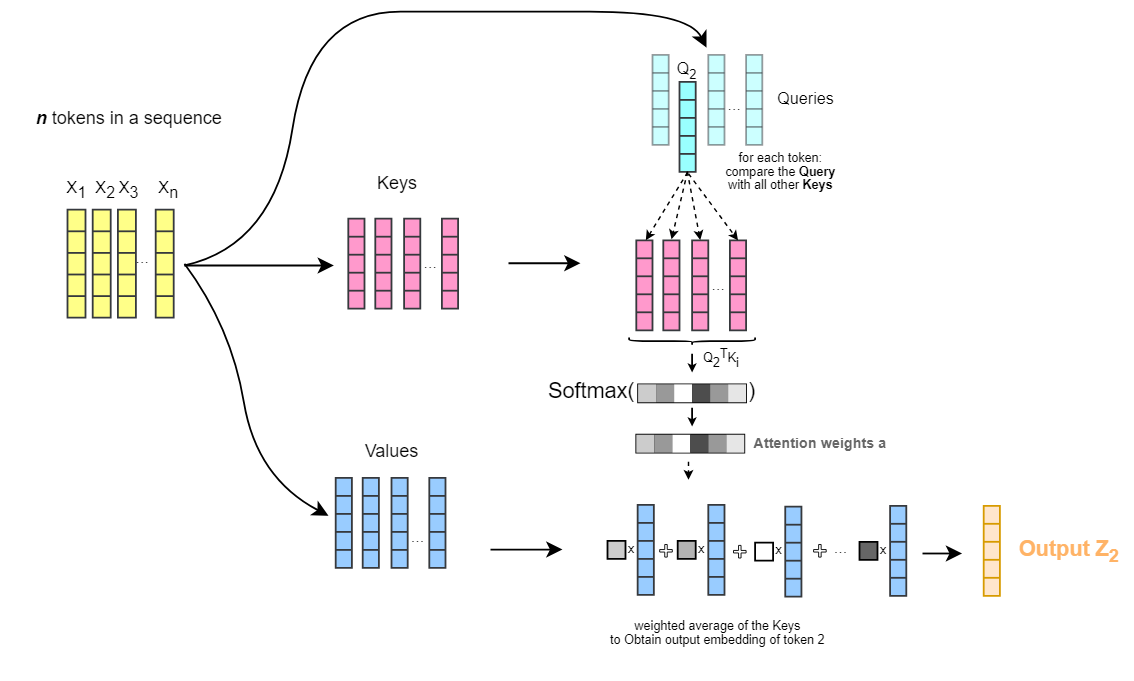
\includegraphics[width=1\textwidth]{2/figures/eqbasmat.png}
		\caption[Diagrama de Q, K, V (queries, keys, values)]{Diagrama de Q, K, V (queries, keys, values).\\
		Fuente: \cite{vaswani2025transformers}. \citetitle{vaswani2025transformers}.}
		\label{2:figeqbasmat}
	\end{center}
\end{figure}

\begin{itemize}
    \item \textbf{Funcionamiento:} La atención se puede aplicar de manera global o local. En el caso de la segmentación de imágenes faciales, por ejemplo, el modelo puede aprender a dar más importancia a las áreas alrededor de los ojos o la frente, donde las arrugas suelen ser más notorias.
    \item \textbf{Beneficio:} Aumenta la precisión de la segmentación al concentrarse solo en las características más relevantes y minimizar el "ruido" de otras regiones no significativas. \parencite{autor2021atencion}
\end{itemize}

\subsubsection{Atención Espacial}  
La atención espacial es un tipo específico de atención que asigna pesos según la ubicación espacial de los elementos dentro de la imagen. Esto permite al modelo resaltar áreas específicas de la imagen que contienen características clave para la segmentación.  

\begin{equation}\label{eq:mapa_atencion_espacial}
    M_s = \sigma(\text{Conv2D}([\text{AvgPool}(F); \text{MaxPool}(F)]))
\end{equation}
\myequations{Mapa de atención espacial}
donde $F$ es el mapa de características, $\sigma$ es la función sigmoide, y $[;]$ denota la concatenación de canales.


\begin{itemize}
    \item \textbf{Funcionamiento:} A través de la atención espacial, el modelo puede identificar patrones en las posiciones de las características de interés, como las arrugas en la zona de la frente o las manchas en la mejilla. Este enfoque es útil cuando las características relevantes están distribuidas de manera no uniforme en la imagen.
    \item \textbf{Aplicación:} Es particularmente eficaz en la segmentación de imágenes faciales, donde las características que deben segmentarse no están siempre en el mismo lugar de la imagen y varían según la persona y la expresión facial. \parencite{autor2020spa}
\end{itemize}

\subsubsection{Atención de Canal}  
La atención de canal se enfoca en las características dentro de los canales de la imagen, es decir, en las distintas representaciones de las características de la imagen que corresponden a las diferentes profundidades o colores de los filtros en una red convolucional. Este tipo de atención permite que la red enfoque su procesamiento en los canales que contienen la información más relevante para la tarea.  

\begin{equation}\label{eq:mapa_atencion_canal}
    M_c = \sigma(\text{MLP}(\text{AvgPool}(F)) + \text{MLP}(\text{MaxPool}(F)))
\end{equation}
\myequations{Mapa de atención de canal}
donde $M_c$ es el mapa de atención de canal, y MLP representa una red neuronal de perceptrón multicapa.


\begin{itemize}
    \item \textbf{Funcionamiento:} En lugar de distribuir el enfoque en toda la imagen, la atención de canal resalta los canales específicos que contienen detalles cruciales, como la textura de la piel o las sombras que definen arrugas o manchas.
    \item \textbf{Beneficio:} Mejora la capacidad del modelo para diferenciar entre características de diferentes intensidades o patrones, lo cual es esencial en imágenes donde la variabilidad de la textura de la piel puede ser un desafío. \parencite{autor2019canal}
\end{itemize}

\subsubsection{Beneficios de las Redes de Atención}  
Las redes de atención proporcionan varios beneficios clave que mejoran la precisión y eficiencia de los modelos de segmentación, especialmente cuando se trabaja con imágenes complejas como las faciales:
\begin{itemize}
    \item \textbf{Precisión mejorada:} Al permitir que el modelo se enfoque en las regiones más importantes de la imagen, las redes de atención ayudan a obtener segmentaciones más precisas y detalladas.
    \item \textbf{Eficiencia en el procesamiento:} Reduciendo el "ruido" o la información irrelevante, las redes de atención aumentan la eficiencia computacional, ya que el modelo dedica más recursos a las áreas clave.
    \item \textbf{Versatilidad:} Las redes de atención se pueden combinar con otros modelos de segmentación, como U-Net o Mask R-CNN, para mejorar aún más la capacidad del modelo para realizar segmentaciones de alta calidad. \parencite{autor2021beneficios}
\end{itemize}

\subsubsection{Ejemplos de Modelos con Atención}  
Existen varios modelos que implementan mecanismos de atención para mejorar la segmentación de imágenes. Algunos ejemplos notables incluyen:
\begin{itemize}
    \item \textbf{Transformer:} 
    
	El modelo Transformer, originalmente propuesto por  \cite{autor2022transformer}, revolucionó el procesamiento de secuencias al introducir el mecanismo de autoatención (\textit{self-attention}) como núcleo de su arquitectura, eliminando la necesidad de componentes recurrentes (RNNs). Aunque inicialmente fue diseñado para tareas de lenguaje natural, su estructura ha sido adaptada exitosamente para procesamiento de imágenes, especialmente en tareas como segmentación semántica y segmentación de instancias.

\paragraph{Arquitectura General:}

La arquitectura del Transformer clásico, como podemos ver en la Figura \ref{2:figarqtrans}, consiste principalmente en:
\begin{itemize}[label=$\bullet$, leftmargin=1em]
    \item Codificador (Encoder): Transforma las entradas en una representación abstracta (\textit{embedding}).
    \item Decodificador (Decoder): Genera la salida basada en la representación interna y la atención.
\end{itemize}
Para imágenes, la variante más usada es Vision Transformer (ViT), donde:
\begin{itemize}[label=$\bullet$, leftmargin=1em]
    \item Una imagen $\mathbf{X} \in \mathbb{R}^{H \times W \times C}$ se divide en pequeños \textit{patches} (sub-imágenes) de tamaño fijo $P \times P$.
    \item Cada \textit{patch} se aplana y se transforma en un vector, formando una secuencia de vectores de entrada similar a las palabras en NLP.
    \item Se añade un \textit{embedding} posicional para retener la información espacial perdida al aplanar los \textit{patches}.
\end{itemize}
El proceso se puede representar así:
\begin{equation}\label{eq:input_sequence_transformer}
    \text{Input Sequence} = \left\{ x_p^1 + E_{\text{pos}}^1, x_p^2 + E_{\text{pos}}^2, \ldots, x_p^N + E_{\text{pos}}^N \right\}
\end{equation}
\myequations{Secuencia de entrada del Transformer para imágenes}
donde $x_p^i$ es el \textit{embedding} del $i$-ésimo \textit{patch} y $E_{\text{pos}}^i$ es su \textit{embedding} posicional.


	\begin{figure}[H]
		\begin{center}
			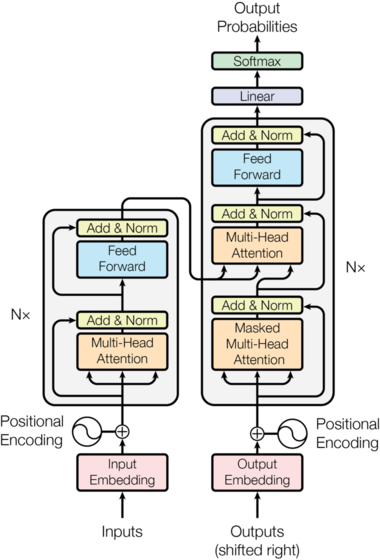
\includegraphics[width=0.45\textwidth]{2/figures/transformers_arquitectura.png}
			\caption[Arquitectura de Transformer]{Arquitectura de Transformer.\\
			Fuente: \cite{autor2022transformer}. \citetitle{autor2022transformer}.}
			\label{2:figarqtrans}
		\end{center}
	\end{figure}
	
	\item \textbf{SENet:} 
	
	SENet, propuesto por \cite{autor2022cnn}, introdujo una estrategia novedosa en las redes convolucionales tradicionales: el módulo de atención de canal llamado Squeeze-and-Excitation (SE) block.

Este módulo no modifica la estructura espacial de las imágenes, sino que aprende a recalibrar dinámicamente la importancia de cada canal de características, ayudando al modelo a enfocarse en los aspectos más relevantes de la representación.
Esta recalibración de canales resulta especialmente útil en tareas de clasificación y segmentación fina, donde detectar características sutiles —como arrugas o manchas faciales— requiere que el modelo preste especial atención a ciertos patrones de textura o color.

\paragraph{Arquitectura del Módulo SE:}

El SE Block se inserta dentro de una red convolucional estándar (por ejemplo, ResNet) y consta de tres etapas principales, como podemos ver en la Figura \ref{2:figarqsenet},:

\textbf{Squeeze (Compresión espacial):}
Reduce cada canal a un único valor mediante una operación de agregación global, usualmente Global Average Pooling (GAP). Esto produce un descriptor de canal que resume la información global de cada mapa de características.
Fórmula:
\begin{equation}\label{eq:squeeze}
    z_c = \frac{1}{H \times W} \sum_{i=1}^{H} \sum_{j=1}^{W} F_c(i,j)
\end{equation}
\myequations{Operación Squeeze}
donde:
\begin{itemize}[label=$\bullet$, leftmargin=1em]
    \item $F_c(i,j)$ es el valor del píxel en la posición $(i,j)$ del canal $c$,
    \item $z_c$ es el valor comprimido del canal $c$.
\end{itemize}

\textbf{Excitation (Recalibración de canales):}
Aprende una relación no lineal entre canales usando una pequeña red neuronal (MLP de dos capas) con activaciones ReLU y sigmoide para generar pesos entre 0 y 1 para cada canal.
Fórmula:
\begin{equation}\label{eq:excitation}
    s = \sigma(W_2 \cdot \delta(W_1 \cdot z))
\end{equation}
\myequations{Operación Excitation}
donde:
\begin{itemize}[label=$\bullet$, leftmargin=1em]
    \item $z$ es el vector comprimido,
    \item $W_1$ y $W_2$ son matrices de pesos aprendibles,
    \item $\delta$ es la función ReLU,
    \item $\sigma$ es la función sigmoide.
\end{itemize}

\textbf{Scale (Reescalado):}
Los pesos aprendidos $s$ son usados para escalar los canales originales del mapa de características:
\begin{equation}\label{eq:scale}
    \tilde{F}_c = s_c \times F_c
\end{equation}
\myequations{Operación Scale}
donde $\tilde{F}_c$ es el canal recalibrado.

	\begin{figure}[H]
		\begin{center}
			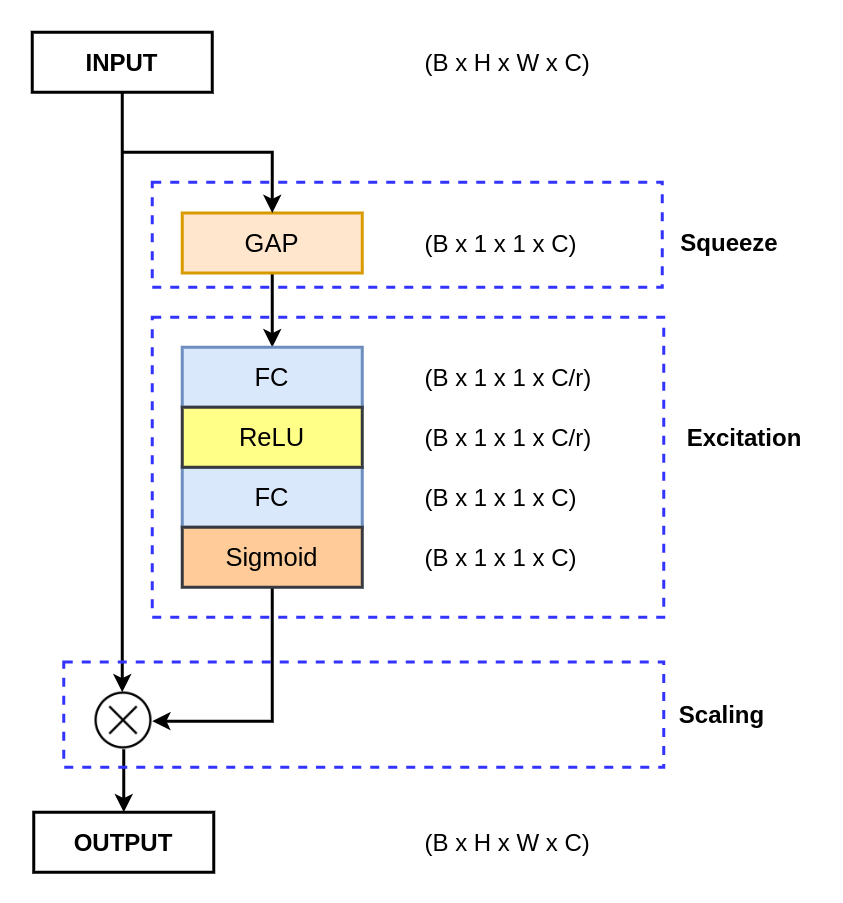
\includegraphics[width=0.65\textwidth]{2/figures/senet.png}
			\caption[Arquitectura de SENet]{Arquitectura de SENet.\\
			Fuente: \cite{autor2022cnn}. \citetitle{autor2022cnn}.}
			\label{2:figarqsenet}
		\end{center}
	\end{figure}

\end{itemize}


\subsection{Modelos Avanzados de Segmentación en Imágenes Médicas}
%
\subsubsection{Comparación entre modelos basados en CNN y modelos híbridos en el contexto dermatológico}
La segmentación de imágenes dermatológicas es crucial para una correcta evaluación clínica y cosmética de la piel, donde las redes neuronales convolucionales (CNN) han demostrado ser eficaces al aprender características relevantes de manera jerárquica y sin necesidad de intervención manual. Sin embargo, las CNN pueden enfrentar desafíos cuando se trata de la segmentación en condiciones de iluminación cambiantes, variabilidad en tipos de piel y características pequeñas como arrugas finas.

Los modelos híbridos, que combinan las capacidades de las CNN con técnicas clásicas de segmentación, ofrecen una alternativa interesante. Estos modelos integran la capacidad de las CNN para aprender representaciones complejas con enfoques más tradicionales como el umbralizado o la segmentación basada en regiones, lo que permite un control más preciso de las áreas de interés, especialmente cuando se requiere segmentar características cutáneas muy específicas. La comparación entre modelos CNN y modelos híbridos ayuda a identificar cuál de estos enfoques es más eficaz dependiendo del tipo de imagen, la complejidad de la tarea de segmentación y los requisitos de precisión.

Por ejemplo, en el análisis de la piel facial, los modelos híbridos podrían combinar las redes convolucionales para la detección de características complejas con métodos tradicionales para afinar los bordes de las regiones segmentadas. Esto puede mejorar significativamente la precisión y robustez del modelo, lo cual es esencial para aplicaciones dermatológicas, donde un pequeño error de segmentación puede afectar el diagnóstico o el tratamiento de afecciones cutáneas. \parencite{hussain2021}

\subsubsection{Métricas de evaluación: Sorensen-Dice, especificidad, precisión, sensibilidad}
Las métricas de evaluación son fundamentales para determinar la calidad y efectividad de los modelos de segmentación, especialmente en el ámbito médico y dermatológico. Entre estas métricas, el índice de Sorensen-Dice es ampliamente utilizado debido a su capacidad para medir la similitud entre las áreas segmentadas y las áreas reales de interés, lo cual es crítico cuando se analiza la precisión de la segmentación de lesiones o características cutáneas. Esta métrica es especialmente útil en la detección de anomalías de la piel, como manchas y arrugas, ya que permite una comparación directa entre la segmentación automática y la segmentación realizada por expertos.

Junto al índice de Sorensen-Dice, otras métricas comunes en la evaluación de modelos de segmentación incluyen la precisión, que mide la exactitud de las regiones segmentadas positivas, y la sensibilidad, que evalúa la capacidad del modelo para detectar correctamente las áreas de interés. La especificidad, por otro lado, mide la capacidad del modelo para identificar correctamente las áreas no relevantes, lo que ayuda a reducir los falsos positivos en la segmentación de imágenes dermatológicas. \parencite{sorensen1948}

\subsubsection{Importancia de la precisión en segmentación de arrugas y manchas para aplicaciones clínicas y cosméticas}
La precisión en la segmentación de características cutáneas como arrugas y manchas es de vital importancia para una evaluación correcta en aplicaciones clínicas y cosméticas. En la práctica clínica, la segmentación precisa permite a los dermatólogos realizar diagnósticos más exactos, detectar signos tempranos de enfermedades de la piel y personalizar los tratamientos para cada paciente. En el ámbito cosmético, la segmentación precisa es esencial para ofrecer recomendaciones personalizadas sobre tratamientos faciales, como la mejora de la textura de la piel o la reducción de manchas y arrugas.

Un modelo de segmentación que no sea preciso puede dar lugar a resultados erróneos, afectando la calidad de los tratamientos recomendados y, por lo tanto, la satisfacción del cliente o del paciente. Además, la segmentación precisa facilita la evaluación del progreso de un tratamiento a lo largo del tiempo, lo que permite a los profesionales de la salud y belleza ajustar sus enfoques terapéuticos de manera más efectiva. \parencite{chuchu2020}

\subsubsection{Variabilidad en tipos de piel y condiciones externas (luz, color)}
Uno de los mayores desafíos en la segmentación dermatológica es la variabilidad en los tipos de piel y las condiciones externas, como la iluminación y los cambios en el color de la piel. Las pieles de diferentes tonos pueden presentar características distintas, como la intensidad del contraste entre la piel y las lesiones, lo que puede dificultar la tarea de segmentación. Además, las condiciones de iluminación, como la luz natural o artificial, pueden alterar la apariencia de las características cutáneas, complicando la segmentación precisa en entornos reales.

Por lo tanto, se necesita el desarrollo de modelos de segmentación más robustos que puedan adaptarse a estas variabilidades. Esto implica entrenar modelos utilizando una amplia variedad de datos, que incluyan diferentes tipos de piel, condiciones de iluminación y otros factores ambientales que puedan influir en la calidad de la imagen y en la precisión de la segmentación. \parencite{zhao2021}


% \subsection{Métricas de Evaluación}  
% Las métricas de evaluación son fundamentales para medir la precisión y eficacia de los modelos de segmentación de imágenes, ya que permiten comparar la segmentación automática generada por el modelo con las segmentaciones de referencia (verdaderas). A continuación se describen las principales métricas utilizadas en este tipo de análisis.

% \subsubsection{Índice de Sorensen-Dice (Dice Coefficient)}  
% El índice de Sorensen-Dice, o simplemente Dice coefficient, es una métrica ampliamente utilizada para evaluar la similitud entre dos conjuntos de datos segmentados. Esta métrica es especialmente útil en problemas de segmentación de imágenes médicas, donde es necesario comparar la segmentación automática con la segmentación de referencia.  
% \begin{itemize}
%     \item \textbf{Fórmula:}  
%     \begin{equation}\label{eq:Índice de Sorensen-Dice}
% 		\text{Dice} = \frac{2|A \cap B|}{|A| + |B|}
% 	\end{equation}
%     donde \( A \) y \( B \) son los conjuntos de píxeles segmentados de la imagen predicha y la imagen real, respectivamente.
%     \item \textbf{Interpretación:} El valor de Dice oscila entre 0 y 1, donde 1 indica una coincidencia perfecta entre las dos segmentaciones, y 0 indica ninguna superposición.
%     \item \textbf{Aplicación:} Es útil para tareas donde se requiere alta precisión en la identificación de áreas segmentadas, como en el análisis de manchas y arrugas en la piel, donde una segmentación precisa es crucial \parencite{autor2020dice}.
% \end{itemize}

% \subsubsection{Coeficiente de Jaccard (Intersection over Union, IoU)}  
% El coeficiente de Jaccard, también conocido como \( \text{Intersection over Union} \) (IoU), es otra métrica popular para evaluar la superposición entre dos conjuntos de segmentación. A diferencia del índice de Dice, IoU mide la relación entre la intersección de los conjuntos de píxeles predichos y reales con respecto a su unión total.  
% \begin{itemize}
%     \item \textbf{Fórmula:}  
%     \begin{equation}\label{eq:Coeficiente de Jaccard}
%     \text{IoU} = \frac{|A \cap B|}{|A \cup B|}
% 	\end{equation}
%     donde \( A \) y \( B \) son los conjuntos de píxeles segmentados de la imagen predicha y la imagen real, respectivamente.
%     \item \textbf{Interpretación:} El valor de IoU también varía entre 0 y 1. Un valor más alto indica una mayor superposición entre los segmentos predichos y reales. IoU es especialmente útil cuando se requiere evaluar la precisión en áreas de segmentación con bordes definidos, como en el análisis de arrugas y poros \parencite{autor2021iou}.
%     \item \textbf{Aplicación:} Es más severo que el índice de Dice, por lo que es adecuado para evaluar tareas donde la precisión en los bordes y las áreas superpuestas es esencial.
% \end{itemize}

% \subsubsection{Precisión (Precision)}  
% La precisión es una métrica que refleja la efectividad del modelo en evitar falsos positivos. Se calcula como la relación entre los verdaderos positivos y el total de elementos que el modelo ha predicho como positivos. En el contexto de la segmentación de imágenes, la precisión mide la exactitud de las regiones predichas como relevantes por el modelo.  
% \begin{itemize}
%     \item \textbf{Fórmula:}  
%     \[
%     \text{Precisión} = \frac{TP}{TP + FP}
%     \]
%     donde \( TP \) son los verdaderos positivos (píxeles correctamente predichos como parte de la característica) y \( FP \) son los falsos positivos (píxeles incorrectamente predichos como parte de la característica).
%     \item \textbf{Interpretación:} Un valor más alto de precisión indica que el modelo es más efectivo en minimizar los falsos positivos, lo cual es crítico en aplicaciones dermatológicas, donde un modelo debe evitar identificar incorrectamente áreas no relevantes como características de la piel.
%     \item \textbf{Aplicación:} Es útil para tareas donde el modelo debe ser riguroso en evitar predecir áreas de la imagen que no pertenecen a la característica de interés, como en el caso de la segmentación de manchas o poros \parencite{autor2019precision}.
% \end{itemize}

% \subsubsection{Entropía Cruzada (Cross-Entropy)}  
% La entropía cruzada es una función de pérdida utilizada comúnmente en problemas de clasificación y segmentación. Mide la disonancia o la diferencia entre la distribución de probabilidad predicha por el modelo y la distribución de probabilidad real (etiquetas verdaderas). En el contexto de la segmentación, la entropía cruzada es utilizada para entrenar el modelo, ya que penaliza las predicciones incorrectas.  
% \begin{itemize}
%     \item \textbf{Fórmula:}  
%     \[
%     \text{Cross-Entropy} = -\sum_{i} y_i \log(p_i)
%     \]
%     donde \( y_i \) es la etiqueta real de la clase \( i \) y \( p_i \) es la probabilidad predicha para la clase \( i \).
%     \item \textbf{Interpretación:} Un valor bajo de entropía cruzada indica que el modelo ha aprendido bien a predecir las clases correctas, es decir, las características de la piel en las imágenes segmentadas. Un valor alto sugiere una mala predicción, lo que indica que el modelo está lejos de la distribución real.
%     \item \textbf{Aplicación:} La entropía cruzada es especialmente útil durante el proceso de entrenamiento para ajustar los parámetros del modelo y garantizar que la segmentación final sea lo más precisa posible, especialmente al tratar con características complejas de la piel como manchas o arrugas \parencite{autor2022crossentropy}.
% \end{itemize}